% This is LLNCSDOC.TEX, the documentation file of
% the LaTeX2e class from Springer-Verlag
% for Lecture Notes in Computer Science, version 2.24
\documentclass[runningheads]{llncs}
% Add PDF bookmarks and metadata
\usepackage[bookmarksopen,
bookmarksopenlevel=1,
bookmarksdepth=2,
pdftex,
pdfauthor={No Author Given},
pdftitle={Instantaneous, Understandable, and Actionable Soundness Checking of Industrial BPMN Models},
pdfsubject={BPMN soundness checking},
pdfkeywords={BPM, BPMN, BPMN analysis, Soundness checking}
]{hyperref}
%
\usepackage{graphicx}
% If you use the hyperref package, please uncomment the following line
% to display URLs in blue roman font according to Springer's eBook style:
% \renewcommand\UrlFont{\color{blue}\rmfamily}

\begin{document}
%
\title{Instantaneous, Understandable, and Actionable Soundness Checking of Industrial BPMN Models}
%
\titlerunning{Instantaneous soundness checking of industrial BPMN models}
% If the paper title is too long for the running head, you can set
% an abbreviated paper title here
%
% \author{Tim Kr\"{a}uter\inst{1}\orcidID{0000-0003-1795-0611} \and
% Adrian Rutle\inst{1}\orcidID{0000-0002-4158-1644} \and
% Harald K\"{o}nig\inst{2,1}\orcidID{0000-0001-6304-6311} \and
% Yngve Lamo\inst{1}\orcidID{0000-0001-9196-1779}}
% \authorrunning{T. Kräuter et al.}
% \institute{Western Norway University of Applied Sciences, Bergen, Norway 
% \email{tkra@hvl.no, aru@hvl.no, yla@hvl.no} \and
% University of Applied Sciences, FHDW, Hanover, Germany\\
% \email{harald.koenig@fhdw.de}}
%
\maketitle              % typeset the header of the contribution
%
\begin{abstract}
TODO
\keywords{
Business Process Modeling \and
Verification \and
BPMN Soundness\and
Quality assurance
}
\end{abstract}

% Up to 16 pages, including everything!

\section{Introduction}
% Why useful?
\cite{fahlandAnalysisDemandInstantaneous2011}
% Claims a lot of problems in workflow models, which can be found using soundness checks.
% Describe the figure and go over all three claims briefly: instantaneous (Definition), understandable (soundness properties are hard to understand for modelers), and actionable (comparable to quick fixes).

% Also add the times measured by other tools for some models. These range into seconds? Would be nice to try the sasme models later.

% Understandable/Visualization is missing in the figure: instantaneous and actionable are there.
\begin{figure}[ht]
	\centering
	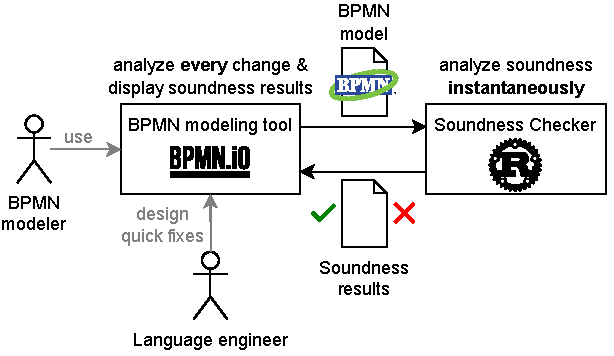
\includegraphics[width=1\textwidth]{images/overview}
	\caption{Overview of the approach}
	\label{fig:overview}
\end{figure}

% What do the results contain? If wrong: Counterexample and problematic elements

% Soundness stuff taken from which adopted it for BPMN
\cite{corradiniClassificationBPMNCollaborations2018}

% One example should be introduced here, which then is picked up throughout the paper.
% Wrong gateway usage?
% Instantaneous: The model checks in 500ms or less.
% Understandable: Highlight problematic elements + show the visualization of a counterexample using that model.
% Actionable: Provide quick fixes that resolve soundness violation --> check if changes fix the property before showing it to the user.

\section{Soundness Checking of BPMN Models}
% Describe soundness checking in general and specifically for BPMN models.

\section{Instantaneous Soundness Checking}
Instantaneous soundness checking is defined as taking 500 ms or less in \cite{fahlandAnalysisDemandInstantaneous2011}.


% Provide empirical evidence that it is instantaneous. Use repositories and synthetic benchmarks with increasing model size and degree of parallelity. --> Maybe in an independent section and link to the results here
% Add all those datasets with artifacts using a Zenodo link --> Artifacts badge

These guys have some benchmarks:
\cite{corradiniFormalApproachAnalysis2021}


\subsection{Growing Model Size}
% Cite my LMCS paper here if already published.
% Briefly recap the method, but we only test in steps of 10.
% Should include those models somewhere

\subsection{Growing Degrees of Parallelism}
% Cite the other paper here with parallelism

\subsection{Industrial Models}
% Check that we can check and analyze models from the model repositories cited anywhere.
% Especially look for models to be "industrial"! --> some in my previous publications were.

\section{Understandable Soundness Checking}

% Highlight directly and instantly in the diagram --> Overlays (and colors)
% Interactive visualization of counterexamples.
\cite{camundaservicesgmbhBpmnjsTokenSimulation2024}

\section{Actionable Soundness Checking}

% Quick fix providers/analysis resolvers/solution strategies/resolution strategies coded for the different soundness properties.
% Custom quick fix providers are also possible in the future with access to model-checking

When possible, we detect errors in the BPMN model and provide an automatic fix similar to quick fixes in IDEs.
Modelers can then select these quick fixes to resolve a specific soundness property.

Since checking soundness is inexpensive, the user can apply the quick fix and instantly get feedback on the changes.
If he is unhappy with the result, a user can undo these changes immediately since each quick fix is a \textit{command} (see command pattern \cite{gammaDesignPatternsElements1995}).
A user might not like a quick fix if it not only fixes a specific property but also has unintended side effects.
For example, it might invalidate a different soundness property.

In the following sections, we describe the implemented resolution strategies for the different soundness properties in detail.
However, we do not expect these strategies to cover all possible resolutions and fit all applications.
Thus, our framework is extensible, so other developers can provide additional or custom resolution strategies (dependency injection, decoupled analysis from handling from showing the errors).
% --> Add before and after figures for each maybe and link to the example demo page hosted somewhere (azure).

\subsection{Safeness} \label{subsec:safeness}
The soundness checker will provide a counter-example and the unsafe sequence flows.
We use this information together with the structure of the BPMN model to find resolutions for \textit{Safeness} violations.
In general, violations can have multiple reasons.

\textbf{(1):} An exclusive gateway with multiple incoming sequence flows activated more than once will lead to multiple tokens at its outgoing sequence flows.

\textbf{(2):} One can also implicitly encode an exclusive gateway, for example, using an activity, by having multiple incoming sequence flows.
Implicitly encoding exclusive gateways is allowed but violates best practices (see lint rule \textit{fake-join} in \cite{camundaservicesgmbhBpmnlint2024}).
Similar to \textbf{(1)}, this leads to unsafe sequence flows if activated more than once.


\textbf{Resolutions for (1):} A straightforward solution is to change the exclusive gateway to a parallel one.
Since the gateway was activated multiple times it indicates that it perhaps should have been a parallel gateway or there was an unintended parallelization before.
Thus, we can analyze the BPMN model and find the parallelization that causes the \textit{Safeness} violation.
If it is a parallel gateway, another solution is to change this parallel gateway to an exclusive one.
So, there are two solutions, but the goal is to have matching gateways.
The parallelization can also be an implicitly encoded parallel gateway, for example, an activity with multiple outgoing sequence flows, which does not comply with best practices but is allowed.
In this case, we can add an exclusive gateway to eliminate the implicit parallelization and achieve matching gateways.
% It would be nice to mention the command here already.

\textbf{Resolutions for (2):} Similarly to \textbf{(1)}, the goal of each quick fix is to obtain matching gateways.
Thus, one solution is to find the parallelization that causes the \textit{Safeness} violation and change it to an exclusive gateway, as described in \textbf{(1)}.
Quick fix \textbf{(a)} in \autoref{fig:safeness} shows this solution, where a parallel gateway is changed to an exclusive one.
We color all changes and additions green in figures, highlighting quick fixes.
Another solution is to remove the implicit exclusive gateway and add a parallel gateway instead, see quick fix \textbf{(b)} in \autoref{fig:safeness}.
The quick fix moves elements automatically to make space to insert the parallel gateway and then reconnects as well as adds sequence flows accordingly.
Even though these are multiple individual operations, we ensured that an undo operation would revert the whole quick fix.
All the implemented quick fixes can be reverted using one simple undo operation.

\begin{figure}[ht]
	\centering
	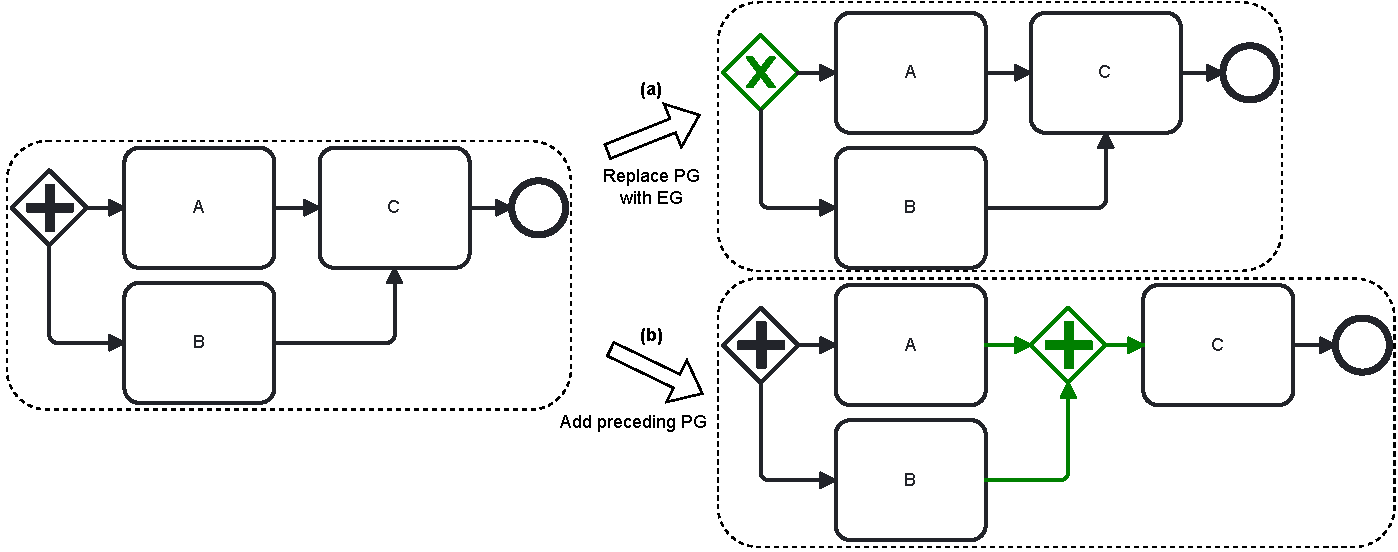
\includegraphics[width=1\textwidth]{images/safeness}
	\caption{Example quick fixes for \textit{Safeness}}
	\label{fig:safeness}
\end{figure}

% TODO: Add demo application and artifacts anonymously.
Our demo application in x contains examples of the Safeness quick fixes and all other soundness properties.

\subsection{Proper Completion}
The soundness checker will provide a counter-example and the end events that consume more than one token.
Violations of \textit{Proper Completion} at a specific end event can have multiple reasons.

\textbf{(1):} An end event might have multiple incoming sequence flows that can hold tokens.
This could be due to a parallelization that is never synchronized.

\textbf{(2):} If there is only one incoming sequence flow, then this sequence flow must be unsafe, i.e., hold more than one token in a possible execution.

\textbf{Resolution for (1):} If multiple incoming sequence flows are the cause, we can add a unique end event for each except the first. 
\autoref{fig:properCompletion} shows an example of this quick fix being applied, where the changed elements are colored in green.
We ensured that an undo operation would revert the quick fix using the command pattern \cite{gammaDesignPatternsElements1995}.

\begin{figure}[ht]
	\centering
	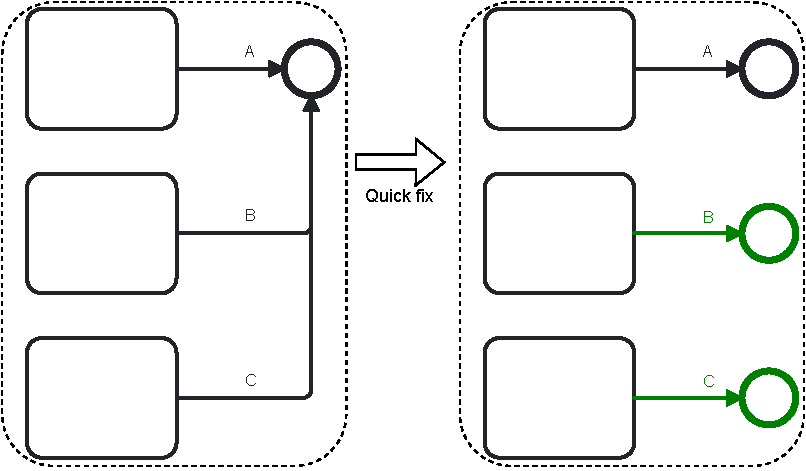
\includegraphics[width=0.7\textwidth]{images/properCompletion}
	\caption{Example quick fix for \textit{Proper Completion}}
	\label{fig:properCompletion}
\end{figure}

\textbf{Resolution for (2):} If a problematic end event only has one incoming sequence flow it must be unsafe.
Thus, other \textit{Safeness} quick fixes can apply, which will also resolve \textit{Proper Completion}, see \autoref{subsec:safeness}.


\subsection{Option to Complete} \label{subsec:optionToComplete}
Violations of \textit{Option to Complete} can have multiple reasons.

\textbf{(1):} A parallel gateway that tries to synchronize multiple incoming sequence flows but never executes can be a problem.

\textbf{(2):} Events that are never triggered but relied upon in the process execution might be another problem.

To know the reason for a given violation, we analyze the counter example provided by the soundness checker.
The counter-example provides a trace that leads to a state in which the process cannot complete.
By analyzing the last state in this trace, i.e., the state in which execution cannot continue, we can determine which element is the cause.
Thus, we can provide quick fixes for the possible reasons.

\textbf{Resolutions for (1):} A straightforward way to fix sequence flow not continuing past a parallel gateway is to change it from parallel to exclusive.
Exclusive gateways do not synchronize, and thus, execution can continue.
\autoref{fig:optionToComplete} \textbf{(a)} shows an example of this quick fix where the replaced gateway is highlighted in green.

\begin{figure}[ht]
	\centering
	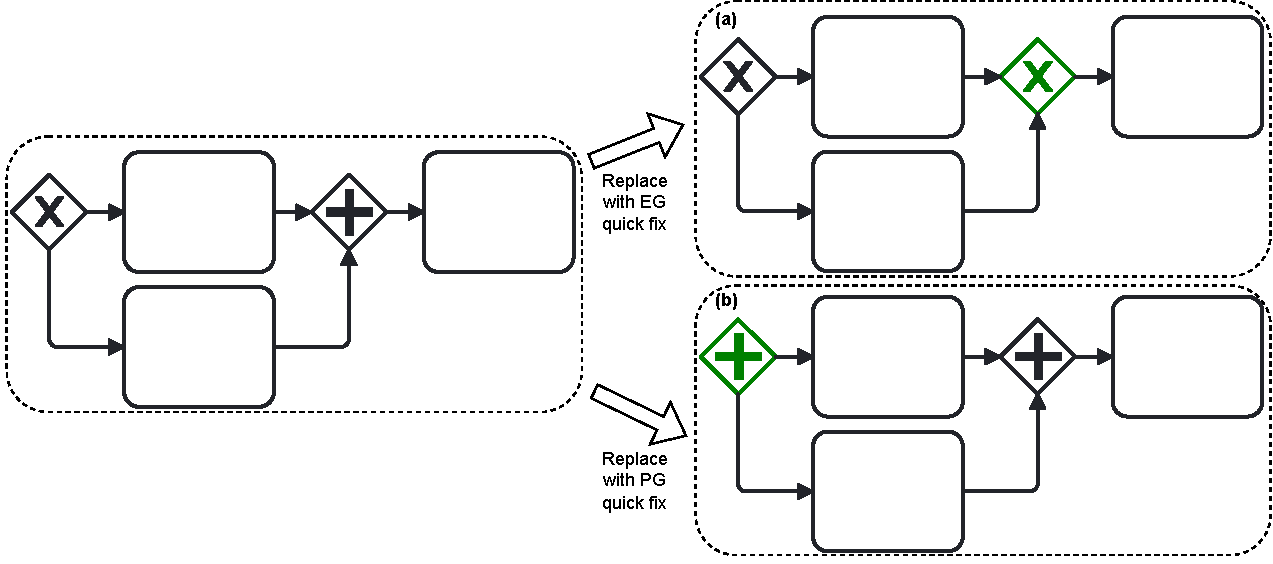
\includegraphics[width=1\textwidth]{images/optionToComplete}
	\caption{Example quick fixes for \textit{Option To Complete}}
	\label{fig:optionToComplete}
\end{figure}

Another way to fix violations is to find the split in the sequence flow, for example, the exclusive gateway in \autoref{fig:optionToComplete}, and make this split a parallelization, see quick fix \textbf{(b)} in \autoref{fig:noDeadActivitiesQuickFix}.
We present both possible resolutions to the user, who can choose the appropriate one.
Similar to the quick fixes 

In the example in \autoref{fig:noDeadActivitiesQuickFix}, it is possible to spot the mismatching gateways.
However, this might not be straightforward in bigger BPMN models with more flow nodes and sequence flows.

\textbf{Resolutions for (2):} We have not yet implemented any quick fixes for events, but many interesting possibilities exist.
For example, for message catch events without incoming message flows, one could add a fitting message flow from a message throw event or send task.
One can use different factors, such as spatial proximity and name similarity, to find the right source of the new message flow.
The idea for any event would be to add the missing trigger.
Finding the most fitting trigger can be done in various ways by analyzing the other elements in the BPMN model.


\subsection{No Dead Activities}
A dead activity might have multiple reasons:

\textbf{(1):} The simplest reason is that the activity is disconnected, i.e., it has no incoming sequence flow.
Disconnected activities must not be dead, but they violate best practices see lint rule \textit{no-disconnected} in \cite{camundaservicesgmbhBpmnlint2024}.

\textbf{(2):} An activity can also be part of the BPMN model that is not reachable during execution because a parallel gateway preceding the activity cannot be executed.
% Could also be behind events that are never triggered.

\textbf{Resolutions for (1)}: If the activity is disconnected, we can propose connecting it to the nearest flow-node.
However, this flow node should not be disconnected or dead itself.
Concretely, we assume modeling from left to the right, such as all the other automatic layout mechanisms in bpmn-js \cite{camundaservicesgmbhBpmnjs2024} to find the leftmost nearest flow-node to connect.
\autoref{fig:noDeadActivitiesQuickFix} shows an example where this quick fix is applied.
As in the other examples, new elements are colored in green.

\begin{figure}[ht]
	\centering
	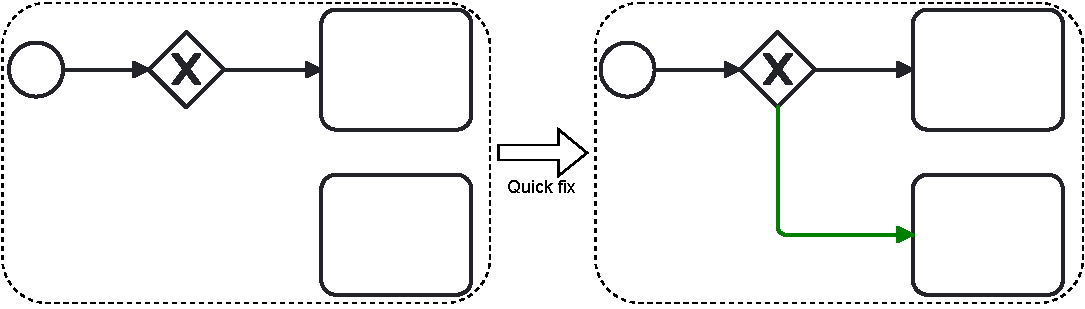
\includegraphics[width=0.6\textwidth]{images/dead}
	\caption{Example quick fix for \textit{No Dead Activities}}
	\label{fig:noDeadActivitiesQuickFix}
\end{figure}

\textbf{Resolutions for (2)}: When the dead activity is connected, this will often lead to processes that cannot terminate, i.e., violate \textit{Option to Complete}.
Thus, other quick fixes can apply, which will also resolve dead activities, see \autoref{subsec:optionToComplete}.

\section{Implementation}

\subsection{Rust}
% Why in Rust?
% Low-level language with modern features.
% Good for CLI tools such as this

% Highlight Rusts speed and safety claims. Maybe cite some papers investigating this. Bottom line: Rust's performance is comparable to C and C++ with better development ergonomics and newer features (less cargo since it is a newer language).
% Zero-overhead abstractions --> related to speed
% Memory-management model in rust (Ownership, borrowing, and lifetimes) --> related to speed and performance
% Zero-copy? --> Currently, we are copying things but still achieve better performance (Tradeoff with readability)

% Reimplement in rust meme

\subsection{BPMN Semantics}
% Describe the runtime model. What is a state? --> Draw a UML diagram
% Describe what the initial state is. --> Could be configurable in the future.
% Describe BPMN semantics with some diagrams for some examples.
% Use a good running example with a modeling error that wasn't used before (double-blind).

\subsection{Description}
% Tool UI with screenshot
\cite{camundaservicesgmbhBpmnjs2024}
% Tool architecture? UI in JS and backend in Rust. --> shown already earlier
% Just the model checker as a CLI app or a CLI that starts the whole thing as a service.

\section{Related Work}

% Different ways of comparison
% 1. BPMN features supported (sub of 2.)
% 2. Capabilities (Which soundness properties are supported, custom properties, counter-example visualization, tool maturity, tool integration, actionability of the tool, etc.)
% 3. Performance using different benchmarks. --> Needs its own paper where everyone can contribute.

\cite{krauterFormalizationAnalysisBPMN2023} % Also add LMCS citation here.

\cite{vangorpVisualTokenbasedFormalization2013}

\cite{corradiniBProVeToolSupport2017,corradiniFormalApproachAnalysis2021}

\section{Limitations \& Threats to Validity}

\section{Conclusion \& Future work}

\bibliographystyle{splncs04} 
\bibliography{bib}

\end{document}
